% arara: xelatex
% arara: xelatex
% arara: xelatex


% options:
% thesis=B bachelor's thesis
% thesis=M master's thesis
% czech thesis in Czech language
% english thesis in English language
% hidelinks remove colour boxes around hyperlinks

\documentclass[thesis=B,english]{FITthesis}[2012/10/20]

\usepackage[utf8]{inputenc} % LaTeX source encoded as UTF-8
% \usepackage[latin2]{inputenc} % LaTeX source encoded as ISO-8859-2
% \usepackage[cp1250]{inputenc} % LaTeX source encoded as Windows-1250

\usepackage{graphicx} %graphics files inclusion
% \usepackage{subfig} %subfigures
% \usepackage{amsmath} %advanced maths
% \usepackage{amssymb} %additional math symbols

\usepackage{dirtree} %directory tree visualisation
\usepackage{color} %VH for comments
\usepackage{csquotes}

\usepackage{todonotes}

\usepackage{amssymb}

\usepackage{algorithm, algcompatible} %for for creating algorithm figures
\algnewcommand\INPUT{\item[\textbf{Input:}]}
\algnewcommand\OUTPUT{\item[\textbf{Output:}]}
\algdef{SE}[DOWHILE]{DO}{DOWHILE}{\algorithmicdo}[1]{\algorithmicwhile\ #1}%

\newcommand{\specialcell}[2][l]{%
\begin{tabular}[#1]{@{}l@{}}#2\end{tabular}}

%\usepackage[main=english,czech]{babel}

% % list of acronyms
% \usepackage[acronym,nonumberlist,toc,numberedsection=autolabel]{glossaries}
% \iflanguage{czech}{\renewcommand*{\acronymname}{Seznam pou{\v z}it{\' y}ch zkratek}}{}
% \makeglossaries

% ------------- Colors abbreviations ------------
\def\cbl{\color{blue}} %VH's suggestions
\def\cre{\color{red}}  %JH's discussion
% % % % % % % % % % % % % % % % % % % % % % % % % % % % % %
% EDIT THIS
% % % % % % % % % % % % % % % % % % % % % % % % % % % % % %

\department{Department of Computer Systems}
\title{ Memory efficient cluster representations in non-metric spaces}
\authorGN{Jaroslav} %author's given name/names
\authorFN{Hlaváč} %author's surname
\author{Jaroslav Hlaváč} %author's name without academic degrees
\authorWithDegrees{Jaroslav Hlaváč} %author's name with academic degrees
\supervisor{Ing. Martin Kopp}
\acknowledgements{THANKS (remove entirely in case you do not with to thank anyone)} %TODO
\abstractEN{Summarize the contents and contribution of your work in a few sentences in English language.}
\abstractCS{V n{\v e}kolika v{\v e}t{\' a}ch shr{\v n}te obsah a p{\v r}{\' i}nos t{\' e}to pr{\' a}ce v {\v c}esk{\' e}m jazyce.} %TODO
\placeForDeclarationOfAuthenticity{Prague}
\keywordsCS{Výběr reprezentantů, Detekce anomálií, Komunitní clusterování, Systém detekce narušení, $\delta$-medoids, Topologický prostor, Párová podobnost} %TODO
\keywordsEN{Representative selection, Network anomaly detection, Community-based clustering, Intrusion detection system, $\delta$-medoids, Topological space, Pair-wise similarity} %TODO
\declarationOfAuthenticityOption{1} %select as appropriate, according to the desired license (integer 1-6)
% \website{http://site.example/thesis} %optional thesis URL


\begin{document}

% \newacronym{CVUT}{{\v C}VUT}{{\v C}esk{\' e} vysok{\' e} u{\v c}en{\' i} technick{\' e} v Praze}
% \newacronym{FIT}{FIT}{Fakulta informa{\v c}n{\' i}ch technologi{\' i}}

\setsecnumdepth{part}
\chapter{Introduction}

There are still many security issues on the Internet even several decades after it became the dominant medium for communication.
Companies all around the world connect more of their infrastructure to the Internet.
Each connected device is an opportunity for attackers.
Security engineers are always inventing new methods to stop the attacks and keep their networks safe and secure.
It is a never-ending race between attackers, trying to overcome new security methods, and defenders, the security personnel, trying to be always one step ahead of the attackers.
This race creates the drive for more and more sophisticated defense mechanisms. \\

Multi-layer defense systems are protecting contemporary networks.
As attackers overcome one layer, there is yet another layer waiting for them.
However, if the attackers succeed to bypass all of them unnoticed, a huge problem can occur.
They can collect user credentials,  exfiltrate data or gain control of devices without anybody's knowledge.
It can take a long time before somebody notices the breach.
A similar thing happened in Marriot International child company Starwood in 2018 \cite{hron2018breaches}.
Names, emails, addresses and credit card numbers of 500 million customers were stolen in an attack that was discovered in 2018 but possibly could have begun as early as in 2014. \\

One of several methods that are used to detect such intrusions is detecting anomalies in the behavior of network hosts - Network Behavioral Anomaly Detection (NBAD).
In NBAD, devices inside of the network are used as probes to gather information about the behavior of the network or individual hosts.
The method then compares the current behavior of the network to a model created from the historical data.
If a significant deviation in behavior occurs, the security team is notified and can act accordingly. \\

It is not uncommon for a company to have tens of thousands of devices and even more.
Straight forward usage of NBAD in these networks is not sufficient to detect breaches successfully.
For example, infection of a single device can be missed in the traffic of a medium sized company.
In order to detect such anomalies, it is needed to focus on smaller parts of the network.
Behavioral clustering of network hosts can be used to separate it into smaller pieces. \\

In Cognitive targeted anomaly detection framework from Cisco behavioral clustering is used to find groups of similar hosts in a network.
Each cluster created consists of hosts that have similar behavior.
The main focus of this work is to find a representation of these clusters that are used to calculate the model behavior.
These cluster prototypes\todo{Can I use the term cluster prototype before first explaining it?} are then updated dynamically as the behavior of the network changes. \\

Four algorithms previously used to represent clusters in computer vision or other fields were studied and modified for usage in Cognitive anomaly detection framework.
They were tested and compared on both real and test datasets. \\

\todo{Chapters and sections will be briefly explained here.}

%The main focus of this work is in representing these clusters found by clustering algorithms.
%Finding representation of clusters in Cognitive targeted anomaly detection framework is made more difficult by the fact, that similarity measure used for clustering does not form a metric space.
%Therefore the focus on methods that can be used for selecting representatives in non-metric spaces. \\
%
%Each cluster can have up to several thousands of hosts.
%Algorithms considered in this thesis were selected based on the following expectations.
%As the hosts are clustered based on their behavior, it is safe to expect that selecting a subset of the cluster can represent its behavior without losing significant information.
%Furthermore having fewer hosts as representatives of each cluster significantly reduce memory usage. \\

%Why use clustering methods in network anomaly detection?
%Why do we need representative selection?
%What are the next sections about?
%
%Automatically grouping similar objects from a given set into clusters is a
%widely used machine learning technique in many fields ranging from
%recommendation engines and social network analysis to image segmentation and
%medical imaging. New applications of this powerfull method are found every year.
%Clustering is also used for Anomaly Detection in computer systems. \par
%In this work I collected 5TODO known methods used in different fields for
%cluster representation. What these methods have in common is possibility to use
%them in spaces where only generic similarity measure exists (these spaces do
%not necessarily need to be metric).

\chapter{Goals}

This work aims to study methods used for the representation of network host behavioral clusters that can be used in Cognitive targeted anomaly detection framework.
Behavioral similarity used for clustering in this framework does not form a metric space, which creates a requirement for algorithms used for representative selection. \\

This thesis should present a method that can be used for finding the cluster prototypes of clusters in non-metric space.
These cluster prototypes represent the whole cluster in a way that is convenient for further computation.
It can be, for example, assigning newly added samples to their corresponding cluster.\\

Networks monitored by Cognitive targeted anomaly detection framework can have up to several hundreds of thousands of hosts which leads to massive clusters.
If the classification of newly added hosts were done by comparing the new host to all others, the memory and time needed for classification would be unmanageable.
That is why the number of representatives selected from each cluster should be kept as small as possible. \\

General methods used for general cluster representation in non-metric spaces should be studied.
From these previously studied methods, the best ones will be selected and implemented.
As part of this thesis, there should also be created a dataset as a benchmark for testing the chosen method.
A further goal is to test the chosen methods on generally used clustering datasets and the created benchmark dataset.
Based on this testing, find the method that suits best for use in this field and incorporates it into the Cognitive targeted anomaly detection framework.
The selected method should be finetuned to get the best possible results in anomaly-detection.

\setsecnumdepth{all}

%========================================CHAPTER==================================

\chapter{Intrusion Detection System}

This chapter focuses on presenting ideas from network security needed to understand the main objective of this thesis.
Different approaches to network intrusion detection systems (IDS) are explained in Section~\ref{sec:ids}.
In Section~\ref{sec:nbad}, the scope is narrowed to network anomaly detection IDS and Section~\ref{sec:challenges}delves deeper into the challenges of it.
Section~\ref{sec:ctadf} serves as an introduction to Cognitive targeted anomaly detection framework used by Cisco.
Methods researched in this thesis were tested on real data collected from Cognitive targeted anomaly detection framework. \\

\section{Types of Intrusion Detection Systems}\label{sec:ids}

An intrusion detection system (IDS) is a security tool designed for identification of unauthorized use or abuse of computer systems by both system insiders and external penetrators \cite{mukherjee1994network}.
IDS that is explicitly designed for monitoring computer network is called Network IDS (NIDS) as in comparison to host IDS and hybrid IDS.
Host IDS focuses on monitoring the internal state of a computer system (e. g. mainframe computer) and its dynamic behavior.
Hybrid IDS combines different techniques including the ones used in a host and network IDS creating an IDS that can leverage information from each of its parts for better intrusion detection.
Examples of NIDS software are \cite{cooper2019bestids} :
\begin{itemize}
    \item Snort
    \item Suricata
    \item Bro Network Security Monitor
\end{itemize}
These systems are used on computer networks to detect and sometimes even prevent attacks that are threats to one of the essential services of such a network.
These basic services are\cite{mukherjee1994network}:
\begin{itemize}
    \item Data confidentiality
    \item Data and communication integrity
    \item Accessibility
\end{itemize}
Attackers try to disrupt these services by accessing confidential information (snooping), manipulating information (data tampering attacks) or disabling access to network services (Denial of Service attacks).
IDS must have multiple components to detect as many of these attacks as possible.
As each kind of intrusion is better detected by a different method, there are several types of IDS \cite{liao2013intrusion}:
\begin{itemize}
    \item \textbf{Signature-based} (knowledge-based): Patterns of known attacks or threats are being compared to captured events for intrusion detection.
    \item \textbf{Anomaly-based} (behavior-based): A static or dynamic model of a given network is created over a period of time, and current network behavior is compared to expected (model) behavior for anomalies.
    \item \textbf{Stateful protocol analysis} (specification-based): The system keeps track of known protocols (e. g., pairing requests with replies) and finding unexpected behavior in these protocols.
\end{itemize}
Cognitive targeted anomaly detection framework combines all of these approaches.
This thesis focuses on the behavior-based part of the framework.

\section{Network Anomaly Detection}\label{sec:nbad}
Network anomaly detection is a method used in Intrusion Detection Systems (IDS) as explained in the previous section.
This method focuses on comparing network host behavior changes in time.
If a change more significant than a certain threshold is observed, network anomaly is detected.
In IDS, when an anomaly is detected, an alert is created to inform the network administrator about what has happened.
This alert can be any kind of message ranging from a syslog message to an email sent to the admin. \\

Host behavior is collected from devices in the network.
There is at least one device (although many times multiple) dedicated for collection of network flows (using NetFlow protocol).
Flow collection is the most widely used method for gathering data on the network.
One network flow is an aggregated information about one connection that consists of source and destination addresses, source, and destination ports, begin and end timestamps for communication and size of data transferred in each direction.
\todo{[RFC2722] citation}
This aggregation of information enables much faster (even real-time) detection of problems on a network as compared to, for example, deep packet inspection (DPI).
DPI is another method used to detect problems in a network.
It focuses on exploring the payload of each packet and is mostly considered unusable.
Not only the majority of traffic is encrypted, but it is also impossible to look into each packet because of the enormous amount of traffic in today's networks. \\

Network flows are collected and then sent via NetFlow protocol to one place where they are stored, and evaluated by detection algorithms.
Network anomaly detection system creates a baseline model of the network behavior, which is then compared to the actual traffic.
Any sudden change is considered to be an anomaly that is reported by the IDS. \\

\section{Challenges of Real-Time Anomaly Detection}\label{sec:challenges}
Even if it was possible to capture all the traffic in the world and use it for anomaly detection, it would still be impossible to achieve 100\% precision.
Not every network host generates enough traffic to create a precise model of its behavior.
Thankfully absolute precision is not the goal of anomaly detection, as it serves as one of many layers of security in computer systems. \\
\todo{Explain better, what is the goal of anomaly detection, Grill Thesis}

That is why models are calculated for whole networks where it is possible to create a model that reflects the behavior of the network.
This method is widely used, and on smaller (several devices) networks it is very efficient.
However, capturing flow data from a big network of thousands of devices can result in too much information.
One can easily miss one infected device generating different traffic.
The noise in the collected data is too high. \\

To give an example, imagine detection of a single infected device, such as a printer in a 10 story office building.
This printer, being a part of a botnet, was ordered to generate traffic for DDoS (Distributed Denial of Service) attacks.
Looking at the traffic of the printer before and after infection it could easily be seen that it increased by several hundred or even thousands of percent.
But an anomaly detection system could hardly notice a change when considering the traffic of the whole office building. \\

If an AD system does not mark malicious traffic as an anomaly, it is considered a false negative.
That is another challenge AD systems are struggling with, to keep the number of missed attacks at 0 or as close to it as possible.\\

One more problem connected to false negatives are the false positives.
A false positive is a network sample of benign network traffic marked as anomalous by the AD system.
For example, if we would have our anomaly detection system set up wrong, it might detect an anomaly every day at 8 AM when workers come to the office, start their computers and download daily email.
Comparing the time window from before 8 AM and after 8 AM would not give us any relevant information.
This problem can be mitigated by setting a window, for which the model is calculated, long enough so that these mistakes do not happen.
There are many other situations when false positive alerts can happen.
Having more than 0 false positives is not that big of a problem as having more than 0 false negatives.
In IDS there is always a way to filter and double check the anomalies.
However,  a network anomaly detection system should avoid a big overhead in false positives as it could overwhelm the system.\\

In conclusion, a good anomaly detection system should detect all anomalies that are somehow connected to malicious behavior while trying to keep the number of false positives alerts as small as possible.
The small number of false positives that are reported is then double-checked in the following layers in the IDS.

\section{Cognitive Targeted Anomaly Detection Framework}\label{sec:ctadf}

Algorithms studied in this thesis are tested as a part of Cognitive Targeted Anomaly Detection Framework which is a part of Cognitive Threat Analytics developed and used by Cisco.
This framework successfully uses community-based clustering on the behavior of each host \cite{kopp2018community}.
The aim is to split the whole network into smaller groups.
Running anomaly detection for each group then yields significantly better results as compared to the traditional whole network approach.
Not only it works better because of community-based clustering, but also because of the ability to adapt dynamically as the network changes.
Thus it is able to incorporate changes that happen on a given network such as adding and removing devices.\\

The method is separated into two phases.
In the initial phase, the state of the network is learned, and an initial model is created.
Then, in the second ongoing phase, the framework dynamically adjusts clusters to the current state of the network. \\

The initial phase starts by collecting 24 hours of traffic from a given network.
Collected data consists of network traffic flows and proxy server logs.
Once the 24-hour period is over, clustering of hosts starts.
Each host is represented by a tuple $h = {S^h, F^h}$, where:
\begin{itemize}
    \item $S^h$ represents set of all visited pairs server:port
    \item $F^h$ represents the frequency of visits of server:port pairs
\end{itemize}
The frequency is defined as:
$$F_s^h = \frac{i}{n}\sum\limits_{1}{n}I(t_i, s, h)\:,$$ where $n$ is the number of time windows, $I$ is the indicator function, which is 1 if the network host $h$ visited the server $s$ in the timewindow $t_i$ and 0 otherwise.
This ratio-based frequency ensures that frequently visited servers (e.g., Google, Facebook) do not overshadow the less frequently visited servers.\\

When each host is represented, the clustering algorithm is started.
A technique called community-based clustering is used to create groups of hosts.
This clustering works for graphs, where communities are more densely connected parts of the graph.
In the words of this NBAD: Those hosts that communicate with similar peers are considered to be in the same community.
Community-based clustering is explained in detail in Section~\ref{sec:cluster_topo}.\\

The density of samples in sets of data is determined by cosine similarity of frequency vectors of two hosts.
Similarity measure between hosts \textit{a} and \textit{b} is defined as:
$$\textrm{cos}(a, b) = \frac{\sum\limits_{s \in S} F_s^a F_s^b} {\sqrt{\sum\limits_{s \in S} (F_s^a)^2} \sqrt{\sum\limits_{s \in S} (F_s^b)^2}}\:,$$
where $F_a$, $F_b$ represent the frequency and $S$ represents the union of sets of servers visited by the network hosts $a$ and $b$. \\

After the clustering is done, only clusters that are bigger than 10 hosts are selected for representative selection.
Smaller clusters are analyzed using a fallback method - host-centered anomaly detection.
For the purpose of this work, we do not consider clusters smaller than 10 hosts. \\

When clusters are determined, $\kappa$ random representatives are selected from each cluster.
Currently, $\kappa$ is an empirically set parameter.
In this thesis, tests were made to improve this random selection method.
A more detailed explanation of this method can be found in \cite{kopp2018community}.\\

After the initial training phase is over and the model is established, data continues to be collected.
Every 4 hours all hosts that are observed are assigned to existing clusters.
At that point, a portion of cluster representatives is replaced by new ones to capture the ever-changing nature of the network data. \\

These clusters are then further used in anomaly detection.
They serve as a foundation for calculating baseline behavior for hosts belonging to it.
If a host is known to belong to a cluster $A$ and its behavior suddenly starts to differ from the behavior of representatives selected for cluster $A$, an anomaly is found and reported further into the NIDS.

%========================================CHAPTER==================================

\chapter{Theoretical Overview}

This chapter introduces a theoretical background to explain clustering methods, the topic of non-metric spaces and the problem of representative selection.

\section{Introduction to Clustering}\label{sec:clust_intro}
As defined in \cite{guttag2016introduction}, clustering is an unsupervised machine learning method that organizes objects into groups so that each group consists of members that are similar in some way.
Without any prior knowledge of the data, this method looks for structures in feature vectors.
Variability can be calculated for each cluster \textit{c}, and it shows how much objects in given cluster differ.
Variability and dissimilarity are two properties defined for a better understanding of the data. \\
Variability is defined as $$ \mathrm{variability}(c) = \sum_{e \in c} \mathrm{distance}(\mathrm{mean}(c), e)^2\:,$$\todo{number equations} where \textit{e} is an object from given cluster.
The distance is a measure that quantifies how far two objects with the same features are. \todo{better wording here}
Many different distance measures are used in clustering.
Several of commonly used ones are:
\begin{itemize}
    \item Euclidean distance
    \item Minkowski distance
    \item Manhattan distance
    \item Cosine similarity
\end{itemize}

Dissimilarity is defined as $$ \mathrm{dissimilarity}(C) = \sum_{c \in C} \mathrm{variability}(c)\:,$$ where $C$ stands for all clusters the data was clustered into.
For clustering, the aim is to keep the dissimilarity of all clusters from the dataset as low as possible.
Given this definition, the best way to cluster every dataset would be to put each object to its cluster.
That would not lead to any reasonable result.
Therefore there is a constraint added for clustering methods.
It can be either the maximum number of clusters or the maximum distance between two clusters. \\

A straightforward example of clustering is a method called agglomerative hierarchical clustering.
Given $N$ objects in a dataset, it creates $N$ clusters - meaning there is a cluster for each object.
The method looks for two closest clusters and merges them into one.
This agglomerative merging continues until the constraint is met, meaning until there is a certain number of clusters or until the distance between closest clusters exceeds a certain threshold.
This method is a greedy algorithm, and therefore it might not result in globally optimal clustering.
Also, the algorithm has a time complexity of $\mathcal{O}(n^2)$.
Therefore, it cannot be used in big datasets. \\

An example of a much faster clustering algorithm that is also greedy is $K$-means. \todo{How to cite that this is only taken from the book, even though rewritten and selected for my purposes.}
The '$K$' in $K$-means stands for the number of clusters that we want to get as a result.
To use this algorithm the number of desired clusters has to be known in advance.
$K$-means randomly chooses $K$ centroids in the space of the dataset and then assigns each point to a centroid.
After creating these clusters, it calculates a new centroid for each cluster and then assigns the points in datasets to the new centroids.
The algorithm stops when the centroids of clusters stop changing.
Figure~\ref{alg:kmeans} shows the pseudocode of $K$-means.
\begin{algorithm}\label{alg:kmeans}
    \caption{K-Means pseudocode}
    \label{k_mean_pseudocode}
    \begin{algorithmic}[1]
        \INPUT set of examples $X$; number of clusters $k$
        \STATE Randomly chose $k$ examples from $X$ as centroids
        \WHILE{True}
            \STATE Create $k$ clusters by assigning each object to the closest centroid
            \STATE Compute $k$ new centroids by averaging objects in each cluster
            \IF{Centroids do not change}
                \STATE \textbf{break}
            \ENDIF
        \ENDWHILE
    \end{algorithmic}
\end{algorithm} \todo{better pseudocode, find better book}

This algorithm is fast, it has time complexity $\mathcal{O}(k \cdot n)$, where $n$ is the number of objects in a dataset and $d$ is the computation time of a distance between two points.
It is the most common clustering algorithm as it typically converges in a few iterations.
For more details about basic clustering algorithms see \cite{guttag2016introduction}.\\

%summary
The clustering as explained in this section has some restrictions that make it inapplicable for anomaly detection in this work.
Firstly the number of clusters is not previously known, so choosing $K$ for $K$-means is not an option, and secondly, the distance measure used does not form a metric space.
Next section delves deeper into what it means when a measure does not form a metric space.

\section{Clustering on Topological Space}\label{sec:cluster_topo}
This section explains the difference between metric and topological space and clustering approaches for topological spaces. \\

A metric space, as defined in \cite{choudhary1992elements}, is a pair $(X, d)$ where $X$ is a set and $d$ is a mapping from  $X \times X \to \mathbb{R}$\todo{ad pripominka, ze by to melo byt NxN, takhle to je popsane v te citovane knize. Prijde mi, ze je to obecnejsi a drzim se toho jak to popsal ten matematik.} which satisfies the following conditions:
\begin{enumerate}
    \item [(i)] $d(x, y) \geq 0$;
    \item [(ii)] $d(x, y) = 0 \iff x = y$;
    \item [(iii)] $d(x, y) = d(y, x)$
    \item [(iv)] $d(x, z) \leq d(x, y) + d(x, z) \mathrm{for} x, y, z \in X$.
\end{enumerate}

The similarity measure that is used in this thesis as explained in section 1.4 \todo{reference} does not fulfill the last point of the definition above. Furthermore, it is a pairwise similarity that forms form a subspace for comparing each pair of samples.
This is why this similarity measure forms a topological space, which is defined according to, e.g. \cite{stahl2014introduction}. \\

Given any set $S$ a topology on $S$ is a family $F ={F_{\alpha} | \alpha \in A}$, where $A$ is some indexing set, each $F_{\alpha}  \subseteq S$\todo{ad poznamka proc je to tady vsunute - je to prima citace z te knihy}, and with the following properties:
\begin{enumerate}
    \item [(i)] The empty set $\emptyset$ is in $F$.
    \item [(ii)] The given set $S$ is in $F$.
    \item [(iii)] The intersection of any two sets of $F$ is in $F$.
    \item [(iv)] The union of any number of sets of $F$ is in $F$.
\end{enumerate}
The ordered pair ($S, F$) is called a topological space. \\

\todo{explain about neighborhoods}

K-Means clustering from the previous section cannot be used in topological space as the centroids do not exist.
In many cases, there is no prior knowledge of k, as is the case in this thesis.
A popular method that is used for clustering in non-metric spaces is called community-based clustering. \\

Community-based clustering detects communities in the data.
A community is a subset of examples in the data, that is densely connected with each other.
One of the ways how to detect communities in a graph is to create a full-adjacency matrix.
This matrix contains all connections between all nodes in the given graph.
Analyzing the matrix then can tell us about the densities in different parts of graphs.\\

Louvain method is a similar approach to clustering when we do not have a simple graph but a set of samples and a pairwise similarity measure.
This method relies on creating a full similarity matrix for the whole dataset and then looking for communities in the data. \\

In Cognitive Targeted Anomaly Detection Framework Louvain method cannot be used directly as calculating the full similarity matrix has a complexity of $\mathcal(n^2)$, which is impossible to calculate for a large network.
That is why an approximative clustering method is used.
This method iteratively samples network hosts and runs the clustering algorithm on the sampled hosts.
Each iteration creates or updates cluster prototypes.
If the data in the current batch fit into a previously prototyped cluster, they are added to it and the cluster prototype is updated.
If samples differ more than a predefined threshold a new cluster prototype is created.

%========================================CHAPTER==================================

\chapter{Representative Selection}

This chapter introduces a theoretical background to explain clustering methods, the topic of non-metric spaces and the problem of representative selection.

\section{Introduction to Clustering}\label{sec:clust_intro}
As defined in \cite{guttag2016introduction}, clustering is an unsupervised machine learning method that organizes objects into groups so that each group consists of members that are similar in some way.
Without any prior knowledge of the data, this method looks for structures in feature vectors.
Variability can be calculated for each cluster \textit{c}, and it shows how much objects in given cluster differ.
Variability and dissimilarity are two properties defined for a better understanding of the data. \\
Variability is defined as $$ \mathrm{variability}(c) = \sum_{e \in c} \mathrm{distance}(\mathrm{mean}(c), e)^2\:,$$\todo{number equations} where \textit{e} is an object from given cluster.
The distance is a measure that quantifies how far two objects with the same features are. \todo{better wording here}
Many different distance measures are used in clustering.
Several of commonly used ones are:
\begin{itemize}
    \item Euclidean distance
    \item Minkowski distance
    \item Manhattan distance
    \item Cosine similarity
\end{itemize}

Dissimilarity is defined as $$ \mathrm{dissimilarity}(C) = \sum_{c \in C} \mathrm{variability}(c)\:,$$ where $C$ stands for all clusters the data was clustered into.
For clustering, the aim is to keep the dissimilarity of all clusters from the dataset as low as possible.
Given this definition, the best way to cluster every dataset would be to put each object to its cluster.
That would not lead to any reasonable result.
Therefore there is a constraint added for clustering methods.
It can be either the maximum number of clusters or the maximum distance between two clusters. \\

A straightforward example of clustering is a method called agglomerative hierarchical clustering.
Given $N$ objects in a dataset, it creates $N$ clusters - meaning there is a cluster for each object.
The method looks for two closest clusters and merges them into one.
This agglomerative merging continues until the constraint is met, meaning until there is a certain number of clusters or until the distance between closest clusters exceeds a certain threshold.
This method is a greedy algorithm, and therefore it might not result in globally optimal clustering.
Also, the algorithm has a time complexity of $\mathcal{O}(n^2)$.
Therefore, it cannot be used in big datasets. \\

An example of a much faster clustering algorithm that is also greedy is $K$-means. \todo{How to cite that this is only taken from the book, even though rewritten and selected for my purposes.}
The '$K$' in $K$-means stands for the number of clusters that we want to get as a result.
To use this algorithm the number of desired clusters has to be known in advance.
$K$-means randomly chooses $K$ centroids in the space of the dataset and then assigns each point to a centroid.
After creating these clusters, it calculates a new centroid for each cluster and then assigns the points in datasets to the new centroids.
The algorithm stops when the centroids of clusters stop changing.
Figure~\ref{alg:kmeans} shows the pseudocode of $K$-means.
\begin{algorithm}\label{alg:kmeans}
    \caption{K-Means pseudocode}
    \label{k_mean_pseudocode}
    \begin{algorithmic}[1]
        \INPUT set of examples $X$; number of clusters $k$
        \STATE Randomly chose $k$ examples from $X$ as centroids
        \WHILE{True}
            \STATE Create $k$ clusters by assigning each object to the closest centroid
            \STATE Compute $k$ new centroids by averaging objects in each cluster
            \IF{Centroids do not change}
                \STATE \textbf{break}
            \ENDIF
        \ENDWHILE
    \end{algorithmic}
\end{algorithm} \todo{better pseudocode, find better book}

This algorithm is fast, it has time complexity $\mathcal{O}(k \cdot n)$, where $n$ is the number of objects in a dataset and $d$ is the computation time of a distance between two points.
It is the most common clustering algorithm as it typically converges in a few iterations.
For more details about basic clustering algorithms see \cite{guttag2016introduction}.\\

%summary
The clustering as explained in this section has some restrictions that make it inapplicable for anomaly detection in this work.
Firstly the number of clusters is not previously known, so choosing $K$ for $K$-means is not an option, and secondly, the distance measure used does not form a metric space.
Next section delves deeper into what it means when a measure does not form a metric space.

\section{Clustering on Topological Space}\label{sec:cluster_topo}
This section explains the difference between metric and topological space and clustering approaches for topological spaces. \\

A metric space, as defined in \cite{choudhary1992elements}, is a pair $(X, d)$ where $X$ is a set and $d$ is a mapping from  $X \times X \to \mathbb{R}$\todo{ad pripominka, ze by to melo byt NxN, takhle to je popsane v te citovane knize. Prijde mi, ze je to obecnejsi a drzim se toho jak to popsal ten matematik.} which satisfies the following conditions:
\begin{enumerate}
    \item [(i)] $d(x, y) \geq 0$;
    \item [(ii)] $d(x, y) = 0 \iff x = y$;
    \item [(iii)] $d(x, y) = d(y, x)$
    \item [(iv)] $d(x, z) \leq d(x, y) + d(x, z) \mathrm{for} x, y, z \in X$.
\end{enumerate}

The similarity measure that is used in this thesis as explained in section 1.4 \todo{reference} does not fulfill the last point of the definition above. Furthermore, it is a pairwise similarity that forms form a subspace for comparing each pair of samples.
This is why this similarity measure forms a topological space, which is defined according to, e.g., \cite{stahl2014introduction}. \\

Given any set $S$ a topology on $S$ is a family $F ={F_{\alpha} | \alpha \in A}$, where $A$ is some indexing set, each $F_{\alpha}  \subseteq S$\todo{ad poznamka proc je to tady vsunute - je to prima citace z te knihy}, and with the following properties:
\begin{enumerate}
    \item [(i)] The empty set $\emptyset$ is in $F$.
    \item [(ii)] The given set $S$ is in $F$.
    \item [(iii)] The intersection of any two sets of $F$ is in $F$.
    \item [(iv)] The union of any number of sets of $F$ is in $F$.
\end{enumerate}
The ordered pair ($S, F$) is called a topological space. \\

\todo{explain about neighborhoods}

K-Means clustering from the previous section cannot be used in topological space as the centroids do not exist.
In many cases, there is no prior knowledge of k, as is the case in this thesis.
A popular method that is used for clustering in non-metric spaces is called community-based clustering. \\

Community-based clustering detects communities in the data.
A community is a subset of examples in the data, that is densely connected with each other.
One of the ways how to detect communities in a graph is to create a full-adjacency matrix.
This matrix contains all connections between all nodes in the given graph.
Analyzing the matrix then can tell us about the densities in different parts of graphs.\\

Louvain method is a similar approach to clustering when we do not have a simple graph but a set of samples and a pairwise similarity measure.
This method relies on creating a full similarity matrix for the whole dataset and then looking for communities in the data. \\

In Cognitive Targeted Anomaly Detection Framework Louvain method cannot be used directly as calculating the full similarity matrix has a complexity of $\mathcal(n^2)$, which is impossible to calculate for a large network.
That is why an approximative clustering method is used.
This method iteratively samples network hosts and runs the clustering algorithm on the sampled hosts.
Each iteration creates or updates cluster prototypes.
If the data in the current batch fit into a previously prototyped cluster, they are added to it, and the cluster prototype is updated.
If samples differ more than a predefined threshold, a new cluster prototype is created.

\section{Representative Selection}

This section focuses on the idea of finding a representation of clusters.
Clustering huge datasets can result in big clusters of several tens of thousands of objects in them.
Computational operations such as assigning new objects to clusters (e. g. $K$-Nearest Neighbors) are dependent on the number of objects in each cluster or the representation of these clusters.
If it was possible to represent these clusters in a different way than keeping all track of all of the objects, further operations on these clusters would run faster. \\

A cluster prototype is a data sample that represents all samples in the data cluster.
According to \todo{ref Introduction to Data Mining}, there are three motivations for finding the most representative cluster prototypes:
\begin{itemize}
    \item Summarization
    \item Compression
    \item Efficient Finding Nearest Neighbors
\end{itemize}
All of these apply to the NBAD aswell.
Therefore, summarizing the behavior of the whole cluster into a cluster prototype is desirable.
As is finding the smallest possible number of prototypes for each cluster for efficient finding nearest neighbors when adding new hosts to their corresponding clusters. \\

\subsection{Definition of Representative Selection for Non-Metric Spaces}\label{sec:def_rep_selection}
Representative selection aims to find a minimal subset of examples from a cluster, that carries sufficient information about the whole cluster.
This problem was well defined in \cite{liebman2015representative} and the following definition is taken from that paper.

Let $S$ be a data set, $d : S \times S \to \mathbb{R} +$ be a distance measure (not necessarily a metric), and $\delta$ be a distance threshold below which samples are considered sufficiently similar.
The task is finding a representative subset $Z \subset S$ that best encapsulates the data.
Two following requirements are imposed on an algorithm for finding a representative subset:
\begin{itemize}
    \item \textbf{Requirement 1}: The algorithm must return a subset $Z \subset S$ such that for any sample $x \in S$, there exists a sample $z \in C$ satisfying $d(x, z) \le \delta$.
    \item \textbf{Requirement 2} : The algorithm cannot rely on a metric representation of the samples in $S$.
\end{itemize}
To compare the quality of different subsets returned by different algorithms, two criteria are measured:
\begin{itemize}
    \item \textbf{Criterion 1}: $|Z|$ - seeking the smallest possible subset $Z$ that satisfies Requirement 1:.
    \item \textbf{Criterion 2}: Representative should best fit the data on average. Given representative subsets of equal size, the preference is on the one that minimizes the average distance of samples from their respective representatives.
\end{itemize}
Criteria 1 and 2 are applied to a representative set solution.
In addition, the following desiderata for a representative selection algorithm are expected.
\begin{itemize}
    \item \textbf{Desideratum 1}: Stable representative selection algorithms are preferred. Let $Z_1$ and $Z_2$ be different representative subsets for dataset $S$ obtained by two different runs of the same algorithm.
Stability is defined as the overlap $\frac{|Z_1 \cap Z_2|}{|Z_1 \cup Z_2|}$      The higher the expected overlap is, the more stable the algorithm is.
This desideratum ensures the representative set is robust to randomization in data ordering or the choices made by the algorithm.
    \item \textbf{Desideratum 2}: The algorithm should be efficient and scale
well for large datasets.
\end{itemize}

This definition of representative selection problem serves well for this paper.

\subsection{Representative Selection in a Metric Space}\label{sec:rep_select_metric}
\todo{Centroid by si mel zavest a vysvetlit vyhody a nevyhody. Centroid muze byt vazeny nebo aritmeticky prumer, to dokazes zapsat vzorcem a bude to hezky vypadat nebo obrazek nebo tak neco. Medoid si vubec nevysvetlil co je.}
A dataset that has the same number of features for each sample and a metric that fulfills all the requisites shown in \todo{reference the definition} is an example of a dataset in a metric space.
Selecting a prototype from this dataset is often best achieved by calculating a centroid for a given cluster.
A centroid can be, for example, the average of all points in the cluster.
If such a centroid is meaningful (it does not fall away from the data), it can be selected as a prototype.
However, if calculated centroid is not meaningful (it falls outside of the dataset), a medoid can be selected as a prototype.
A medoid is the most representative point of a cluster.

\subsection{Representative Selection in a Topological Space}\label{sec:rep_select_arbitrary}
Clearly, the concept of centroid explained in the previous section cannot be used to solve the problem of finding a representative in an arbitrary space (i.e., topological space).
Medoids, of course, can be selected for datasets in arbitrary spaces. \\

$K$-Medoids algorithm that uses the concept of medoids instead of centroids that are used in the $K$-Means algorithm.


\todo{general approaches}

There are not many well-known approaches to solve this problem.
The one that is used in this thesis is explained in \cite{liebman2015representative}.
They took the main ideas of $K$-Means clustering and transformed them for usage in a non-metric space with a pair-wise similarity measure.
Instead of stating the $K$ in advance they state a parameter  $ 0 \leq \delta \leq 1$ that serves as a constraint.
Then they separate the cluster into subclusters based on this parameter.
Each of these subclusters is represented by a medoid.
A set of these medoids then serves as a cluster prototype for the whole cluster.
This method is explained in greater detail in the Section~\ref{subsec:delta_medoids}.

\section{Algorithms Relevant for Topological Space}\label{sec:relevant_methods}
Based on the previously explained approaches for finding representatives of clusters in non-metric, spaces the following methods were chosen, tested and compared as a part of this thesis.
\begin{itemize}
    \item Random selection
    \item Greedy Selection
    \item Delta-Medoids One-Shot
    \item Delta-Medoids \todo{citations}
\end{itemize}

\subsection{Random Selection}\label{subsec:random_select}

Random selection algorithm serves as a baseline to measure the improvement as it is the method currently used in Cognitive targeted anomaly detection framework.
It selects a given number of representatives from the cluster randomly. \\

In clusters dense clusters, selecting random samples from each cluster leads to undesired noise.
However as experimental results presented in \cite{kopp2018community} in the domain of computer networks the density of clusters is not significant.
It, of course, depends on each network, but given the best practices in segmentation of networks, the overlaps in clusters are not expected to be great. \\

For this thesis, the random selection algorithm serves as a baseline in comparing the results to other methods.

\subsection{Greedy Selection}\label{subsec:greedy_select}
\todo{obrazky sem a do dalsi sekce}
The greedy selection algorithm is a straightforward algorithm that selects a random sample from the set as the first representative.
Then it looks for the most different sample in the rest of the dataset.
Once the desired sample is found, the algorithm removes all neighboring samples with at least the similarity of $\delta$ from the set.
Then it looks for other dissimilar samples until the whole set is represented. \\ \todo{pseudocode}

The speed of this algorithm depends on the sparsity of the given set.
In the worst case scenario, all points would be selected as representatives while always calculating the distance to each remaining sample in the set. Then it would reach the time complexity of $\mathcal{O}(n^2)$.

\subsection{$\delta$-Medoids}\label{subsec:delta_medoids}
The two following algorithms were first eplained in \cite{liebman2015representative}.
They were tested on two different problems that also use clustering in non-metric space - computing distance of two musical segments and comparing trajectories of objects.\\

$\delta$-Medoids algorithm tries to find a minimal subset of points that are needed to cover the cluster with only one given constraint, that distance of the representatives would be at least $\delta$.
There are two versions of this algorithm.
One-shot version is faster but less precise than the full $\delta$-medoids algorithm.

\subsection{$\delta$-Medoids One-Shot}

The idea behind this algorithm is to go through the dataset looking for representatives that differ at least by the given parameter $\delta$ from each previously selected representatives.
By taking this approach, it can in one iteration over data find the representatives that are certain to differ by $\delta$ from each other. \\

The algorithm is shown in Figure~\ref{alg:delta_medoids_one_shot}, this algorithm is optimized for better memory efficiency as opposed to the version in the cited paper.
The main ideas remain the same, only keeping track of clusters that the points are assigned to is removed for this one-shot version.

\begin{algorithm}\label{alg:delta_medoids_one_shot}
    \caption{$\delta$-Medoids One-shot}
    \label{delta_medoids_one_shot}
    \begin{algorithmic}[1]
        \INPUT data $x_0$ ... $x_m$, required distance $\delta$
        \STATE Initialize \textit{representatives} = $\emptyset$
        \FOR{$i = 0$ \textbf{to} $m$}
            \STATE Initialize \textit{dist} = $\infty$
            \FOR{\textit{rep} in \textit{representatives}}
                \IF{$d(x_i, rep) \le dist$}
                    \STATE $dist = d(x_i, rep)$
                \ENDIF
            \ENDFOR
            \IF{$dist > \delta$}
                \STATE add $x_i$ to \textit{representatives}
            \ENDIF
        \ENDFOR
    \end{algorithmic}
\end{algorithm}


The choice of the first representative strongly influences the selection of the medoids to represent the cluster.
In some cases, this one-shot approach could be misleading.

\subsection{$\delta$-Medoids}

The full version of the algorithm runs a one-shot algorithm multiple times.
Each time it goes through the dataset it selects a better medoid than before.
Once two passes through the data do not change any medoid, the algorithm stops.
This algorithm is shown in Figure~\ref{alg:delta_medoids_full}.\\

This approach is slower, as the main routine from one shot algorithm has to be run multiple times.
\todo{Mention convergence of the algorithm.}
On the other hand, it is able to select better medoids, thus getting rid of the difficult choice of the first representative to select.

\begin{algorithm}\label{alg:delta_medoids_full}
    \caption{$\delta$-Medoids}
    \label{delta_medoids_full}
    \begin{algorithmic}[1]
        \INPUT data $x_0$ ... $x_m$, required distance $\delta$
        \STATE t = 0
        \STATE Initialize $representatives_{t_0} = \emptyset$
        \STATE Initialize \textit{clusters} = $\emptyset$
        \DO
            \STATE $t = t + 1$
            \FOR{$i = 0$ \textbf{to} $m$}
                \STATE Initialize \textit{dist} = $\infty$
                \STATE Initialize \textit{representative = null}
                \FOR{\textit{rep} in \textit{representatives}}
                    \IF{$d(x_i, rep) \le dist$}
                        \STATE \textit{representative = rep}
                        \STATE $dist = d(x_i, rep)$
                    \ENDIF
                \ENDFOR
                \IF{$dist \le \delta$}
                    \STATE add $x_i$ to $cluster_{representative}$
                \ELSE
                    \STATE \textit{representative = $x_i$}
                    \STATE Initialize $cluster_{representative} = \emptyset$
                    \STATE ad $x_i$ to $cluster_{representative}$
                    \STATE add $cluster_{representative}$ to \textit{clusters}
                \ENDIF
            \ENDFOR
            \STATE Initialize $representatives_t = \emptyset$
            \FOR{\textit{cluster} in \textit{clusters}}
                \STATE $representative = \textrm{argmin}_{s \in cluster} (\sum\limits_{x \in cluster}{d(x,s) : d(x,s) \le \delta)}$
                \STATE add \textit{representative} to $representatives_t$
            \ENDFOR
        \DOWHILE{$representatives_t = representatives_{t-1}$}
    \end{algorithmic}
\end{algorithm} \todo{add the hack for better results}

%========================================CHAPTER==================================

\chapter{Datasets}\label{ch:datasets}

This chapter explains the implementation and testing of selected methods in multiple different scenarios.
In the first section, algorithms for selected methods are listed and explained in detail.
The following section serves as a list of used datasets ranging from general to more specific ones.
The last section of this chapter talks about the tests that were run.
It also explains why the choice of these tests.

\section{Datasets}\label{sec:datasets}
The task of cluster representation in non-metric spaces generally is not necessarily connected only to the Security field.
That is why the selected algorithms were tested on artificially created datasets, clustering datasets previously used in literature and on specific data collected from a real network.
Datasets that are needed for testing methods from this thesis have to be labeled.
That means that each sample in the dataset must be assigned into a cluster so that when the representation for each cluster is found and samples are assigned to clusters, it is possible to doublecheck if the assignment was right.
There are not many labeled datasets that have a lot of samples in each cluster and have the right features for testing. \todo{what does it mean right features, how to better write this}
That is why for complex testing datasets from picture recognition field were used for general testing of methods before going into the area of computer networks.

\subsection{Datasets Created for this Work}

These datasets were created to test the specific properties of tested methods.
The datasets created are the following:
\begin{itemize}
    \item Blobs 3D
    \item Overlap
    \item Circles 3D
    \item Moons
\end{itemize}
All of these datasets are in space of two or three dimensions.
They can be easily visualized on graphs and nicely show some of the specific properties of implemented algorithms.\todo{add pictures}
Similarity measure used in these datasets was Euclidean distance. \\

The Blobs datasets are very easy to represent with a centroid and were tested whether and how much points is needed to represent them using methods explained in Chapter X. \todo{Link to chapter} The Overlap dataset consists of 3 clusters in shapes of blocks.
These blocks partly overlap to test how selected algorithms cope with overlapping clusters. Noisy Circles and Noisy Circles 3D are datasets are one of the hardest datasets to represent even by methods that are designed specifically for metric space.
These two datasets were chosen to test the resistance to noise in selecting representatives.
There are two clusters as shown in figure X. \todo{add figure}

\subsection{Image Recognition Datasets}
One of the best-documented areas of clustering is the area of image recognition.
That is why two datasets from this area were chosen for measuring the precision and complexity of each method.
Both of them are labeled datasets of features collected from digits written by human hand. \\

The Pen-Based Recognition of Handwritten Digits Data Set \cite{dua1998pendigit} consists of 10922 samples with 16 attributes.
Each sample represents features collected from a handwritten digit.
Each digit is represented by a little bit more than a thousand samples.
Features represent coordinate information about the digits as they were written on a $500\times500$ pixel frame.
This dataset is split to train dataset (70\%) and test dataset (30\%).

The Multiple Features Data Set \cite{dua1998pendigit} consist of \todo{explain how is it different} \todo{add MNIST}

\subsection{Real Network Dataset}
Real network traffic captured from a company with approximately 20k employees.
The capture is from 24 hours of a working day a consists of \todo{count flows} flows.
This dataset was created from proxy logs in that company following the workflow explained in section x \todo{Link section.}. \\

%========================================CHAPTER==================================

\chapter{Experiments}
In this chapter each experiment that was run.
Each section is dedicated to one experiment.
For each experiment, the motivation, experimental setup, results and conclusion are listed.

All experiments were made in Jupyter Notebook technology using Python 3.7 kernel.
For loading data from files and storing them in memory was used the Pandas library version 0.23.4\todo{link to documentation}.
These technologies were chosen due to this thesis's experimental nature, as the goal was to produce a prototype solution for this problem.

\section{Experiment 1}\label{sec:exp1}\todo{name differently than Experiment?}

The first experiment was run on easily the data specifically created for this thesis.
It served as a sanity check of the proposed methods.
The methods that were explained in the previous chapter\todo{make reference} are designed to work in non-metric space but they still work in a metric space.
Using them on metric data and visualizing the results helped a lot to check the assumptions about results experimentally.
Also, the need for selection of few representatives from each dataset was tested.
It is expected, for these simple clusters, not to exceed 30 selected representatives.

\subsection{Experimental Setup}
Datasets used for this experiment were:
\begin{itemize}
    \item Blobs 3D
    \item Overlap
    \item Moons
    \item Noisy Circles 3D
\end{itemize}

All 4 algorithms were run.
The $\delta$ was estimated as \todo{how is median at lower ten percent called, put it to maths} times 1.05 from distances from one point in the data to all of the others.

\subsection{Results}

The results for each dataset are listed below.
\textbf{Blobs 3D}

\begin{table}[]
\begin{tabular}{l|lllll}
\hline
 \textbf{Cluster} & \specialcell{\textbf{All}\\ \textbf{Samples}} & \specialcell{\textbf{Greedy}\\ \textbf{Selection}} & \specialcell{\textbf{$\delta$-Medoids}\\ \textbf{One-Shot}} & \specialcell{\textbf{$\delta$-Medoids}\\ \textbf{Full}} & \specialcell{\textbf{Random}\\ \textbf{Selection}} \\ \hline
A & 400 & 21 & 23 & 23 & 23 \\
B & 400 & 17 & 20 & 20 & 20 \\
C & 400 & 19 & 20 & 20 &20  \\ \hline
\end{tabular}
\caption{Number of selected representatives for Blobs 3D dataset}
\end{table}

\begin{figure}
   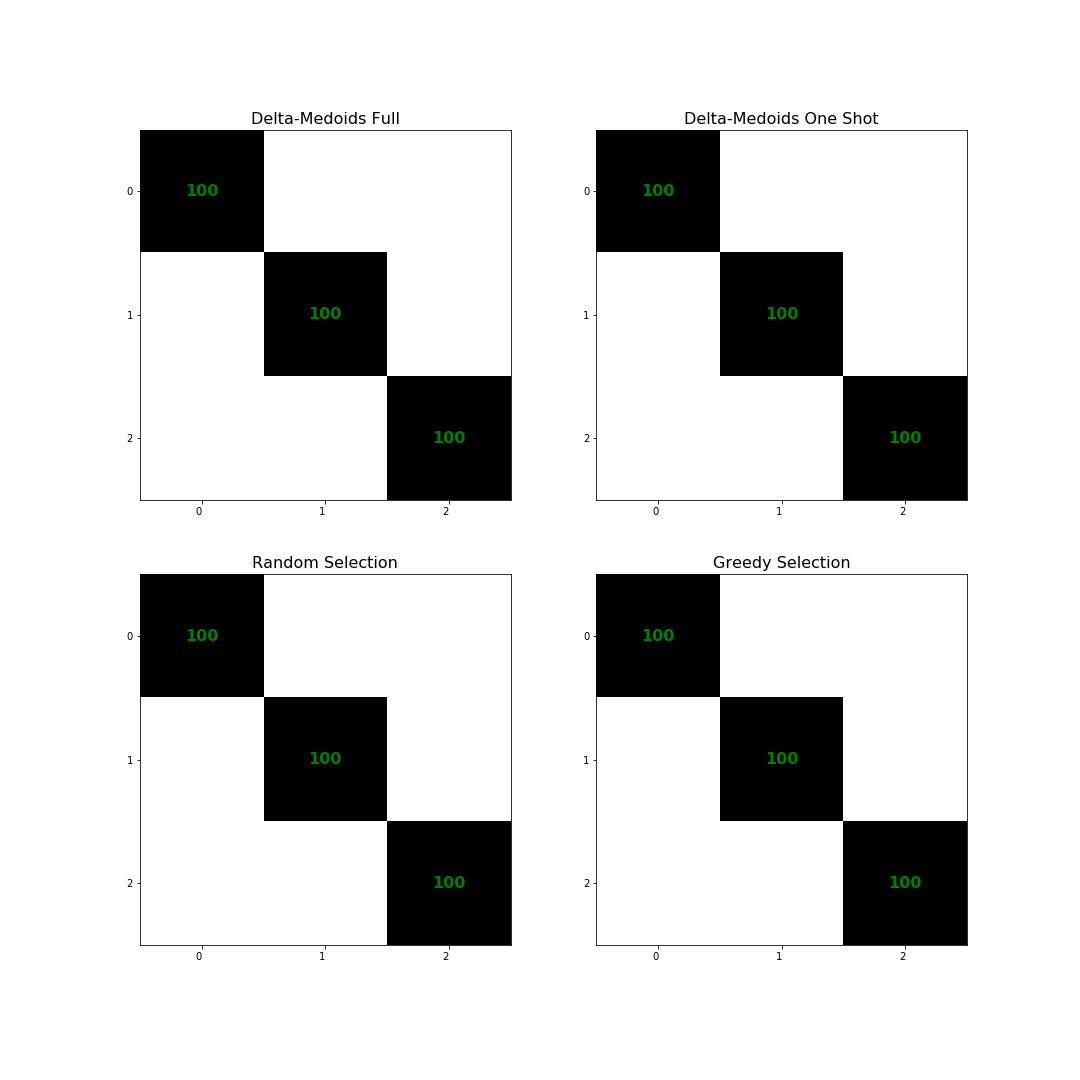
\includegraphics[width=\linewidth]{img/exp1_blobs.png}
  \label{img:exp1_blobs}
  \caption{Confusion matrices for Blobs 3D dataset}
\end{figure}

\textbf{Overlap}

\begin{table}[]
\begin{tabular}{l|lllll}
\hline
 \textbf{Cluster} & \specialcell{\textbf{All}\\ \textbf{Samples}} & \specialcell{\textbf{Greedy}\\ \textbf{Selection}} & \specialcell{\textbf{$\delta$-Medoids}\\ \textbf{One-Shot}} & \specialcell{\textbf{$\delta$-Medoids}\\ \textbf{Full}} & \specialcell{\textbf{Random}\\ \textbf{Selection}} \\ \hline
A & 800 & 25 & 23 & 23 & 23 \\
B & 960 & 26 & 21 & 21 & 21 \\
C & 640 & 22 & 24 & 24 & 24  \\ \hline
\end{tabular}
\caption{Number of selected representatives for Overlap dataset}
\end{table}

\begin{figure}
   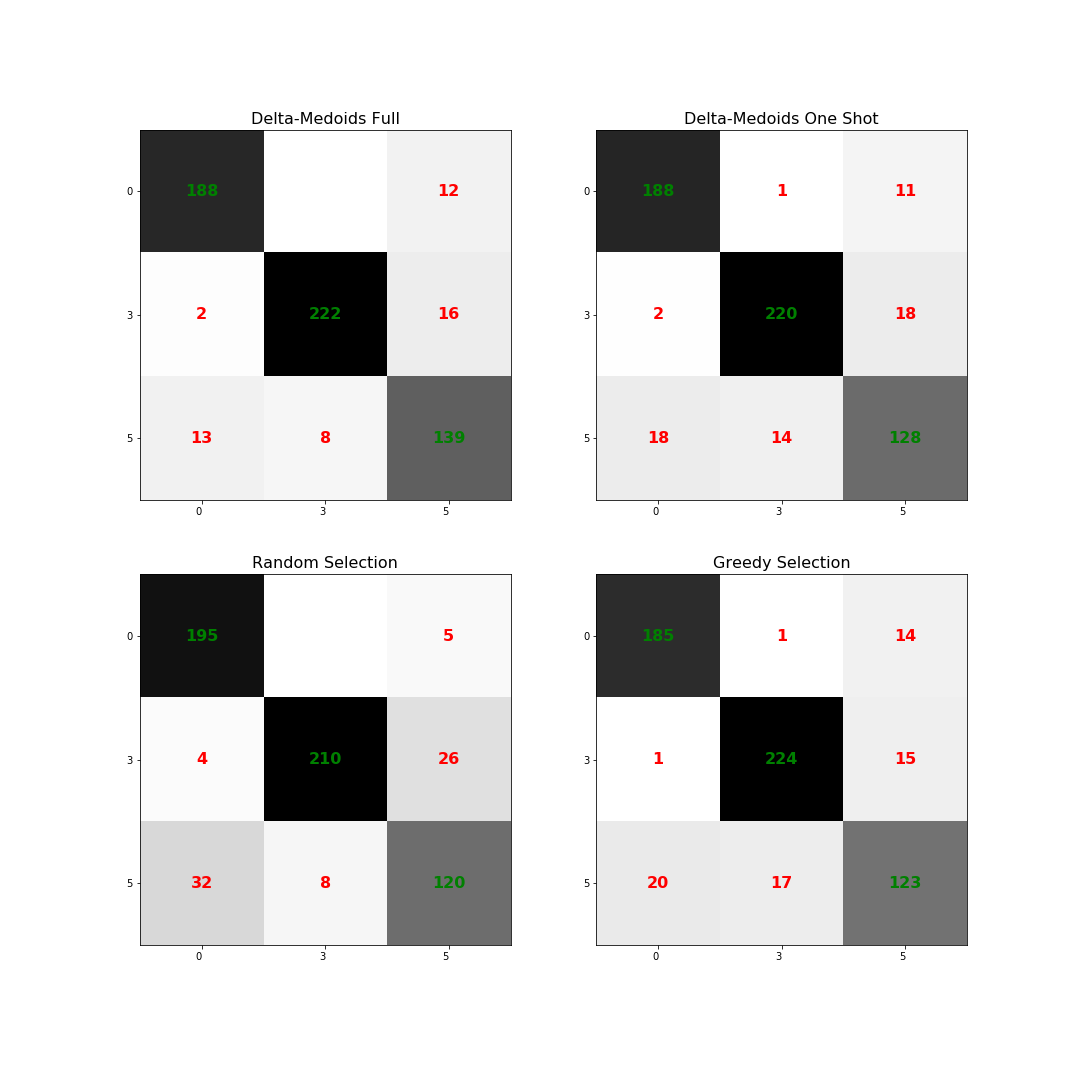
\includegraphics[width=\linewidth]{img/exp1_overlap.png}
  \label{img:exp1_overlap}
  \caption{Confusion matrices for Overlap dataset}
\end{figure}

\textbf{Moons}

\begin{table}[]
\begin{tabular}{l|lllll}
\hline
 \textbf{Cluster} & \specialcell{\textbf{All}\\ \textbf{Samples}} & \specialcell{\textbf{Greedy}\\ \textbf{Selection}} & \specialcell{\textbf{$\delta$-Medoids}\\ \textbf{One-Shot}} & \specialcell{\textbf{$\delta$-Medoids}\\ \textbf{Full}} & \specialcell{\textbf{Random}\\ \textbf{Selection}} \\ \hline
A & 600 & 18 & 19 & 19 & 19 \\
B & 600 & 19 & 18 & 18 & 18 \\ \hline
\end{tabular}
\caption{Number of selected representatives for Moons dataset}
\end{table}

\begin{figure}
   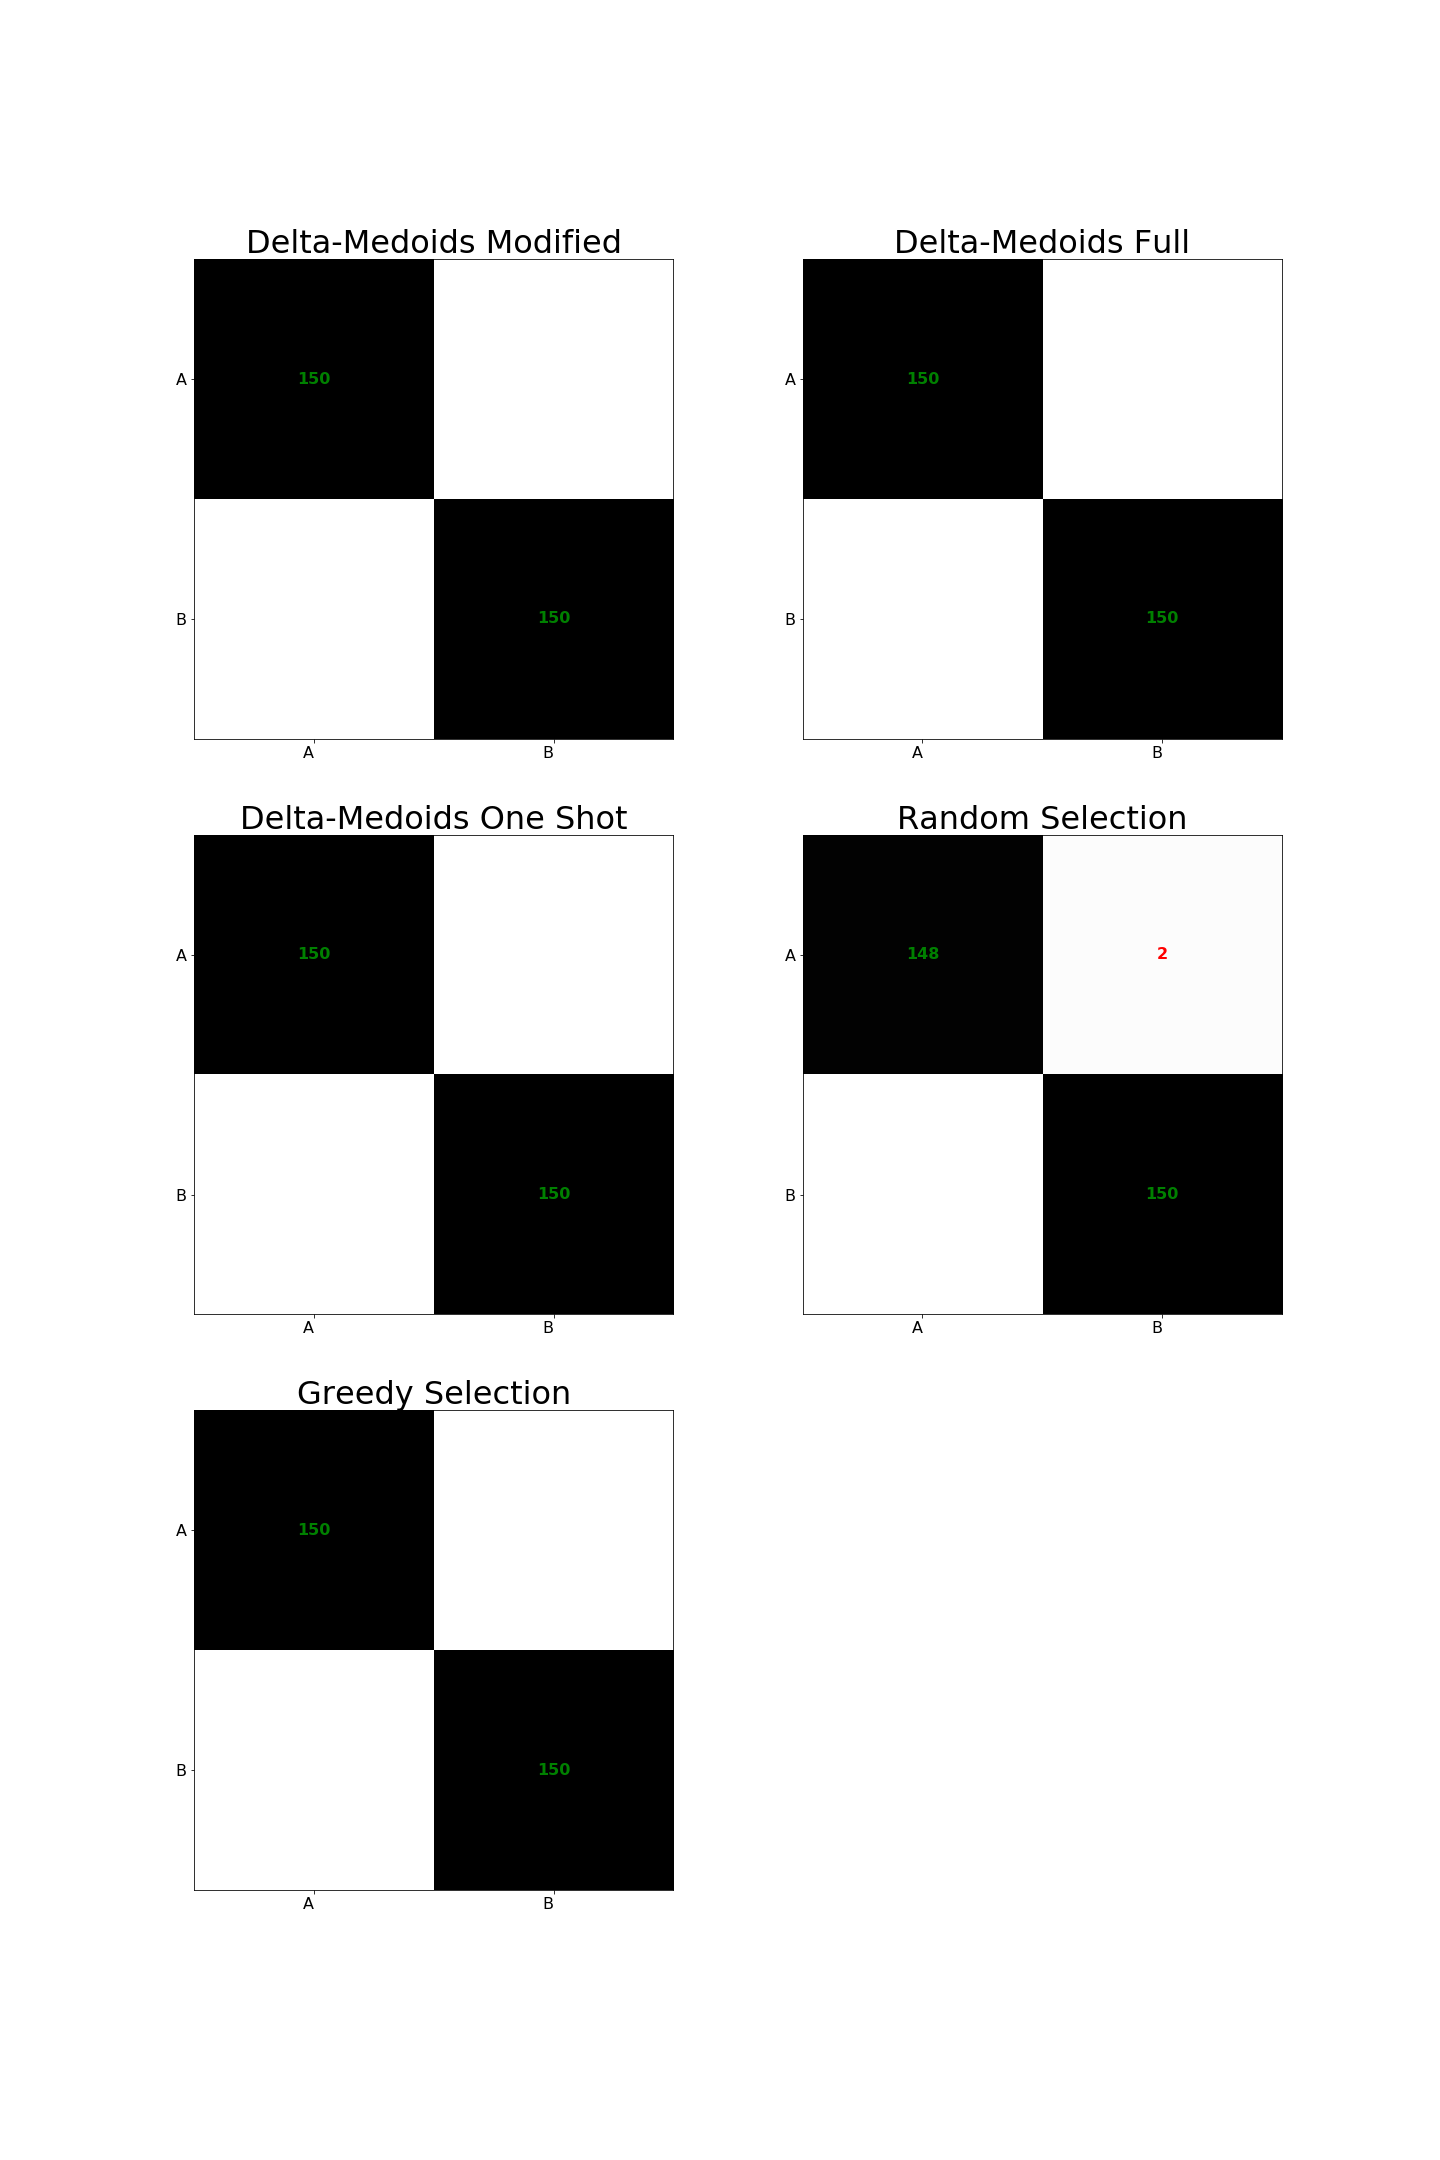
\includegraphics[width=\linewidth]{img/exp1_moons.png}
  \label{img:exp1_moons}
  \caption{Confusion matrices for Moons dataset}
\end{figure}

\textbf{Circles}

\begin{table}[]
\begin{tabular}{l|lllll}
\hline
 \textbf{Cluster} & \specialcell{\textbf{All}\\ \textbf{Samples}} & \specialcell{\textbf{Greedy}\\ \textbf{Selection}} & \specialcell{\textbf{$\delta$-Medoids}\\ \textbf{One-Shot}} & \specialcell{\textbf{$\delta$-Medoids}\\ \textbf{Full}} & \specialcell{\textbf{Random}\\ \textbf{Selection}} \\ \hline
A & 600 & 14 & 14 & 14 & 14 \\
B & 600 & 8 & 7 & 7 & 7 \\ \hline
\end{tabular}
\caption{Number of selected representatives for Circles dataset}
\end{table}

\begin{figure}
   \includegraphics[width=\linewidth]{img/exp1_circles.png}
  \label{img:exp1_circles}
  \caption{Confusion matrices for Circles dataset}
\end{figure}


\subsection{Conclusion}
At first glance, all the confusion matrices look almost perfect and as expected.
The number of representatives selected did not exceed 30 in any cluster.
The number of missed classification is low even in overlapping or complex datasets.
However, when the results were visualized for one cluster, the delta medoids algorithm did not result in expected selection.
As can be seen on Figure~\ref{img:blobs_border_select}, the algorithm picked the samples on the edge of the dataset that did not cover many points in their neighborhoods.
\begin{figure}
   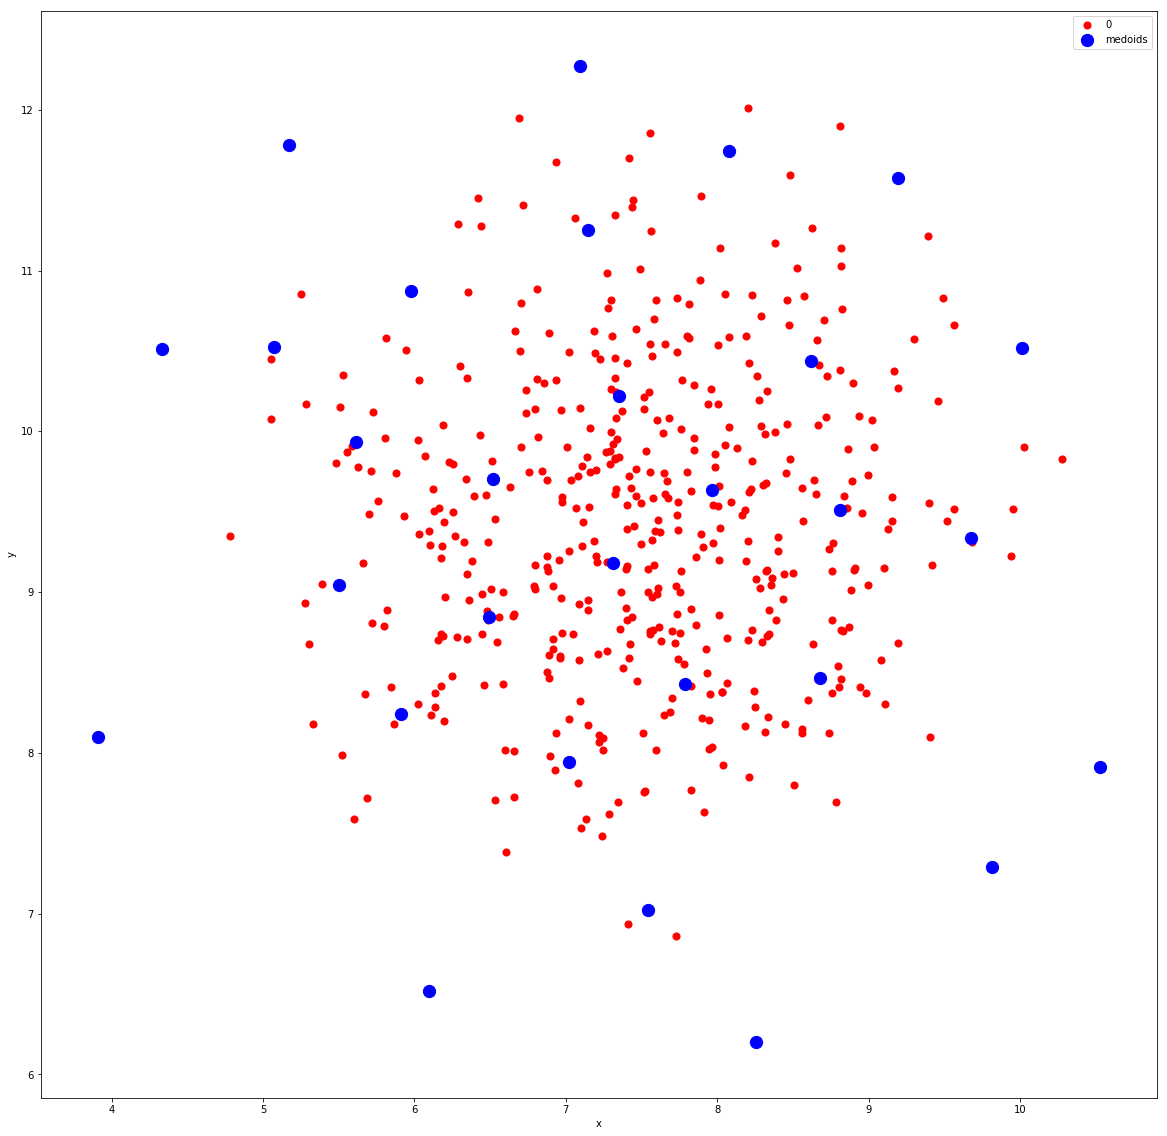
\includegraphics[width=\linewidth]{img/delta_medoids_select.png}
  \label{img:blobs_border_select}
  \caption{$\delta$-Medoids choosing the border samples of a cluster}
\end{figure}
Selecting the border samples clearly was not intended and the $\delta$-Medoids algorithm had to select only the relevant samples.
The relevance of a representative was determined to the number of points that fit into its $\delta$-neighborhood. \todo{where to list the changes, here or in the theoretical chapter, theory better I think}

\section{Experiment 2}\label{sec:exp2}

This experiment was run to test the changes made in the $\delta$-Medoids algorithm.
It was updated not to select the border samples, as is explained in section\todo{ref the section where I explain it}.

\subsection{Experimental Setup}
Datasets used for this experiment were:
\begin{itemize}
    \item Blobs 3D
    \item Overlap
    \item Moons
    \item Noisy Circles 3D
\end{itemize}

All 4 algorithms were run.
The $\delta$ was estimated as \todo{how is median at lower ten percent called, put it to maths} times 1.05 from distances from one point in the data to all of the others.

\subsection{Results}

The results for different methods are listed below.
\textbf{Blobs 3D}

\begin{table}[]
\begin{tabular}{l|lllll}
\hline
 \textbf{Cluster} & \specialcell{\textbf{All}\\ \textbf{Samples}} & \specialcell{\textbf{Greedy}\\ \textbf{Selection}} & \specialcell{\textbf{$\delta$-Medoids}\\ \textbf{One-Shot}} & \specialcell{\textbf{$\delta$-Medoids}\\ \textbf{Full}} & \specialcell{\textbf{Random}\\ \textbf{Selection}} \\ \hline
A & 400 & 23 & 24 & 24 & 24 \\
B & 400 & 21 & 22 & 22 & 22 \\
C & 400 & 20 & 21 & 21 & 21 \\ \hline
\end{tabular}
\caption{Number of selected representatives for Blobs 3D dataset}
\end{table}

\begin{figure}
   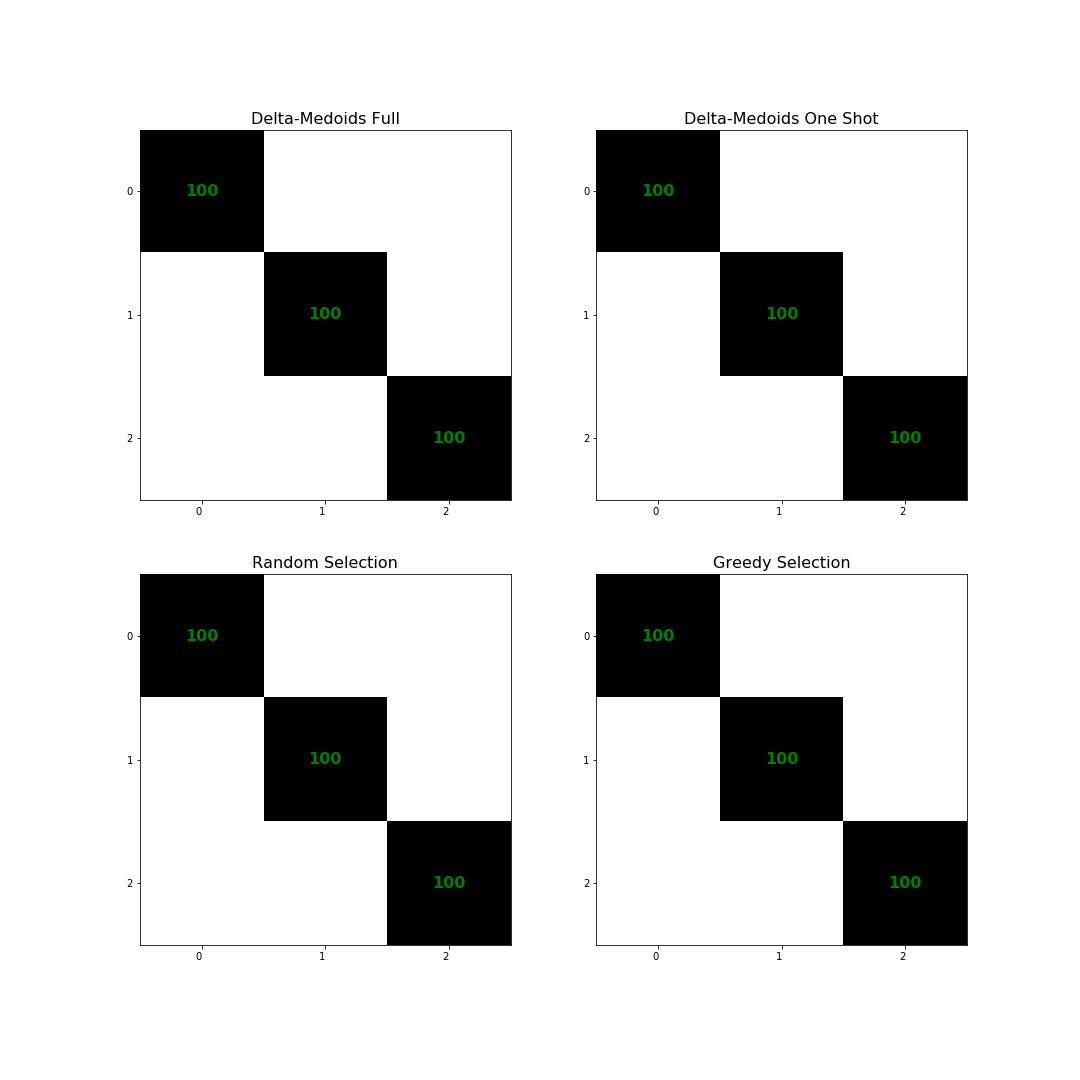
\includegraphics[width=\linewidth]{img/exp2_blobs.png}
  \label{img:exp2_blobs}
  \caption{Confusion matrices for Blobs 3D dataset}
\end{figure}

\textbf{Overlap}

\begin{table}[]
\begin{tabular}{l|lllll}
\hline
 \textbf{Cluster} & \specialcell{\textbf{All}\\ \textbf{Samples}} & \specialcell{\textbf{Greedy}\\ \textbf{Selection}} & \specialcell{\textbf{$\delta$-Medoids}\\ \textbf{One-Shot}} & \specialcell{\textbf{$\delta$-Medoids}\\ \textbf{Full}} & \specialcell{\textbf{Random}\\ \textbf{Selection}} \\ \hline
A & 800 & 22 & 21 & 21 & 21 \\
B & 960 & 21 & 20 & 20 & 20 \\
C & 640 & 19 & 19 & 19 & 19  \\ \hline
\end{tabular}
\caption{Number of selected representatives for Overlap dataset}
\end{table}

\begin{figure}
   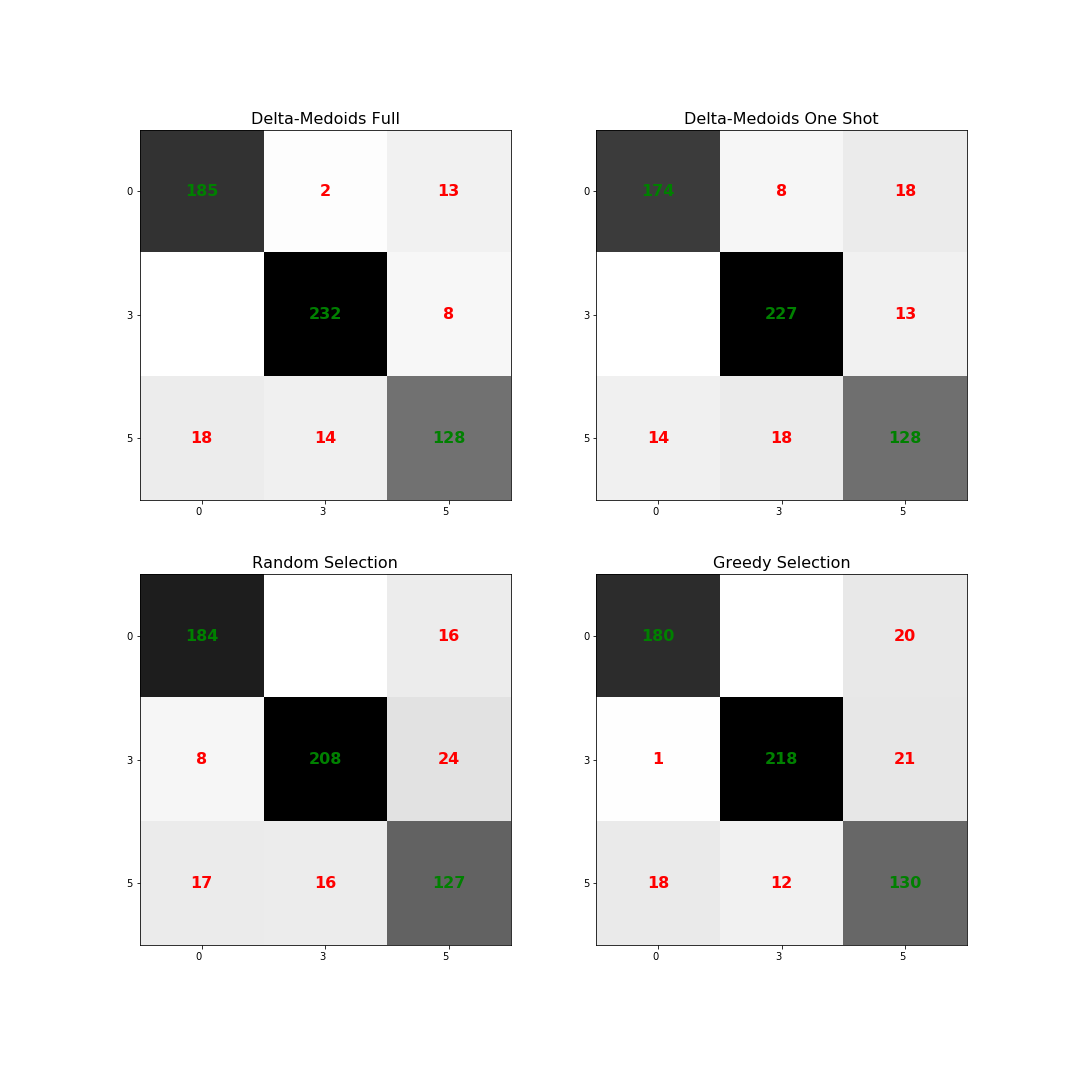
\includegraphics[width=\linewidth]{img/exp2_overlap.png}
  \label{img:exp2_overlap}
  \caption{Confusion matrices for Overlap dataset}
\end{figure}

\textbf{Moons}

\begin{table}[]
\begin{tabular}{l|lllll}
\hline
 \textbf{Cluster} & \specialcell{\textbf{All}\\ \textbf{Samples}} & \specialcell{\textbf{Greedy}\\ \textbf{Selection}} & \specialcell{\textbf{$\delta$-Medoids}\\ \textbf{One-Shot}} & \specialcell{\textbf{$\delta$-Medoids}\\ \textbf{Full}} & \specialcell{\textbf{Random}\\ \textbf{Selection}} \\ \hline
A & 600 & 21 & 18 & 18 & 18 \\
B & 600 & 16 & 20 & 20 & 20 \\ \hline
\end{tabular}
\caption{Number of selected representatives for Moons dataset}
\end{table}

\begin{figure}
   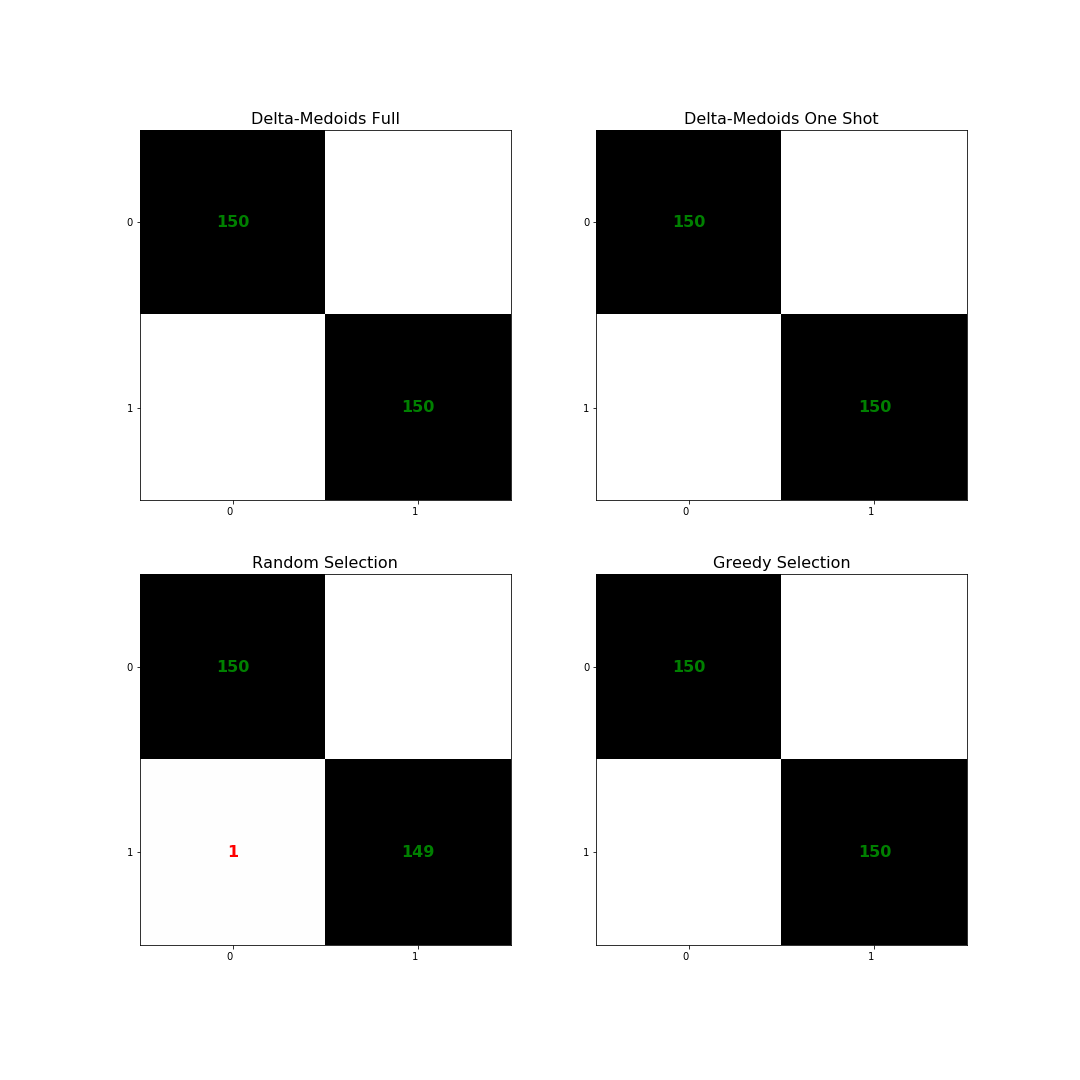
\includegraphics[width=\linewidth]{img/exp2_moons.png}
  \label{img:exp2_moons}
  \caption{Confusion matrices for Moons dataset}
\end{figure}

\textbf{Circles}

\begin{table}[]
\begin{tabular}{l|lllll}
\hline
 \textbf{Cluster} & \specialcell{\textbf{All}\\ \textbf{Samples}} & \specialcell{\textbf{Greedy}\\ \textbf{Selection}} & \specialcell{\textbf{$\delta$-Medoids}\\ \textbf{One-Shot}} & \specialcell{\textbf{$\delta$-Medoids}\\ \textbf{Full}} & \specialcell{\textbf{Random}\\ \textbf{Selection}} \\ \hline
A & 600 & 15 & 15 & 15 & 15 \\
B & 600 & 8 & 8 & 8 & 8 \\ \hline
\end{tabular}
\caption{Number of selected representatives for Circles dataset}
\end{table}

\begin{figure}
   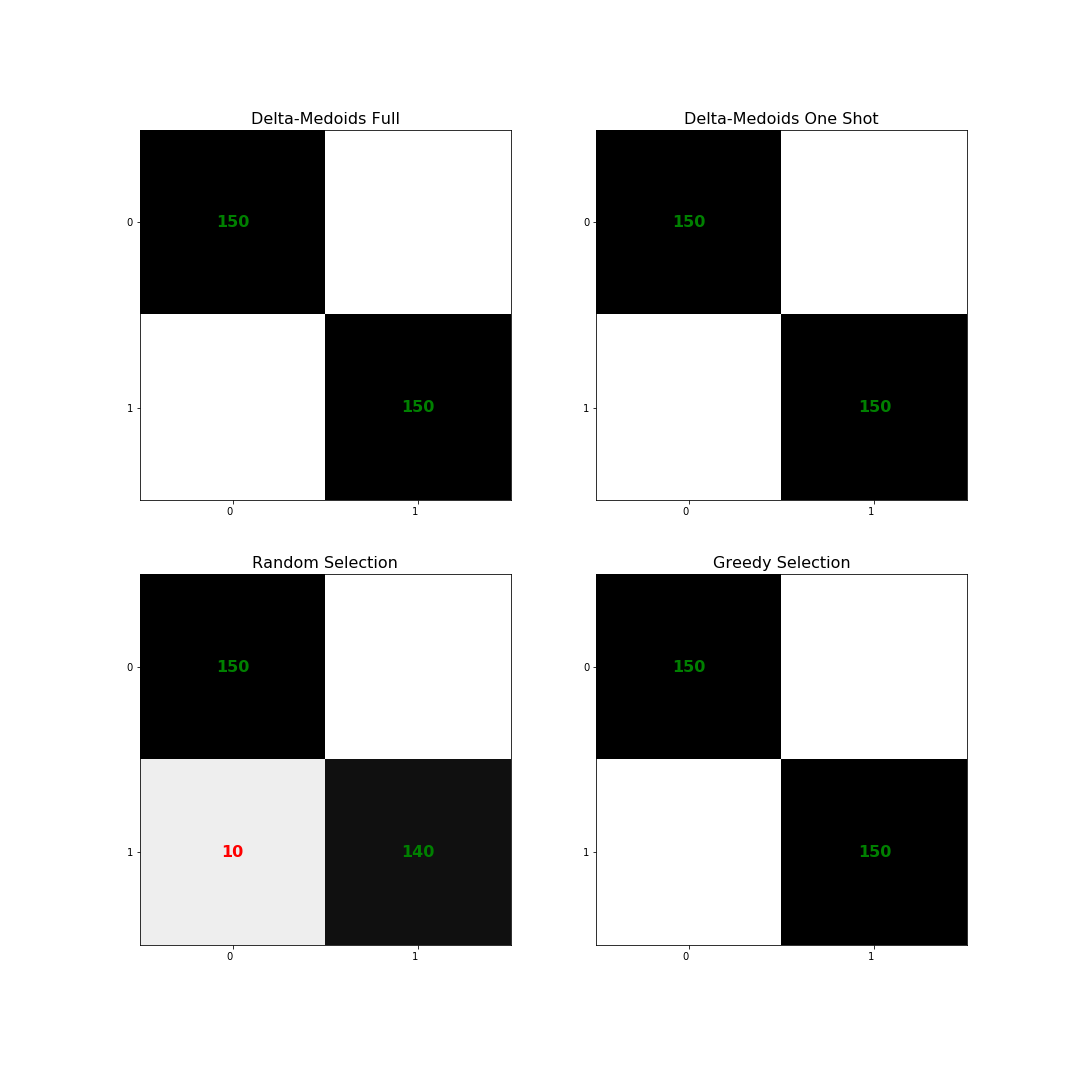
\includegraphics[width=\linewidth]{img/exp2_circles.png}
  \label{img:exp2_circles}
  \caption{Confusion matrices for Circles dataset}
\end{figure}


\subsection{Conclusion}

The results of this experiment empirically supported the expected result of not selecting the border samples from a dataset as can be seen on Figure~\ref{img:blobs_good_select}
\begin{figure}
  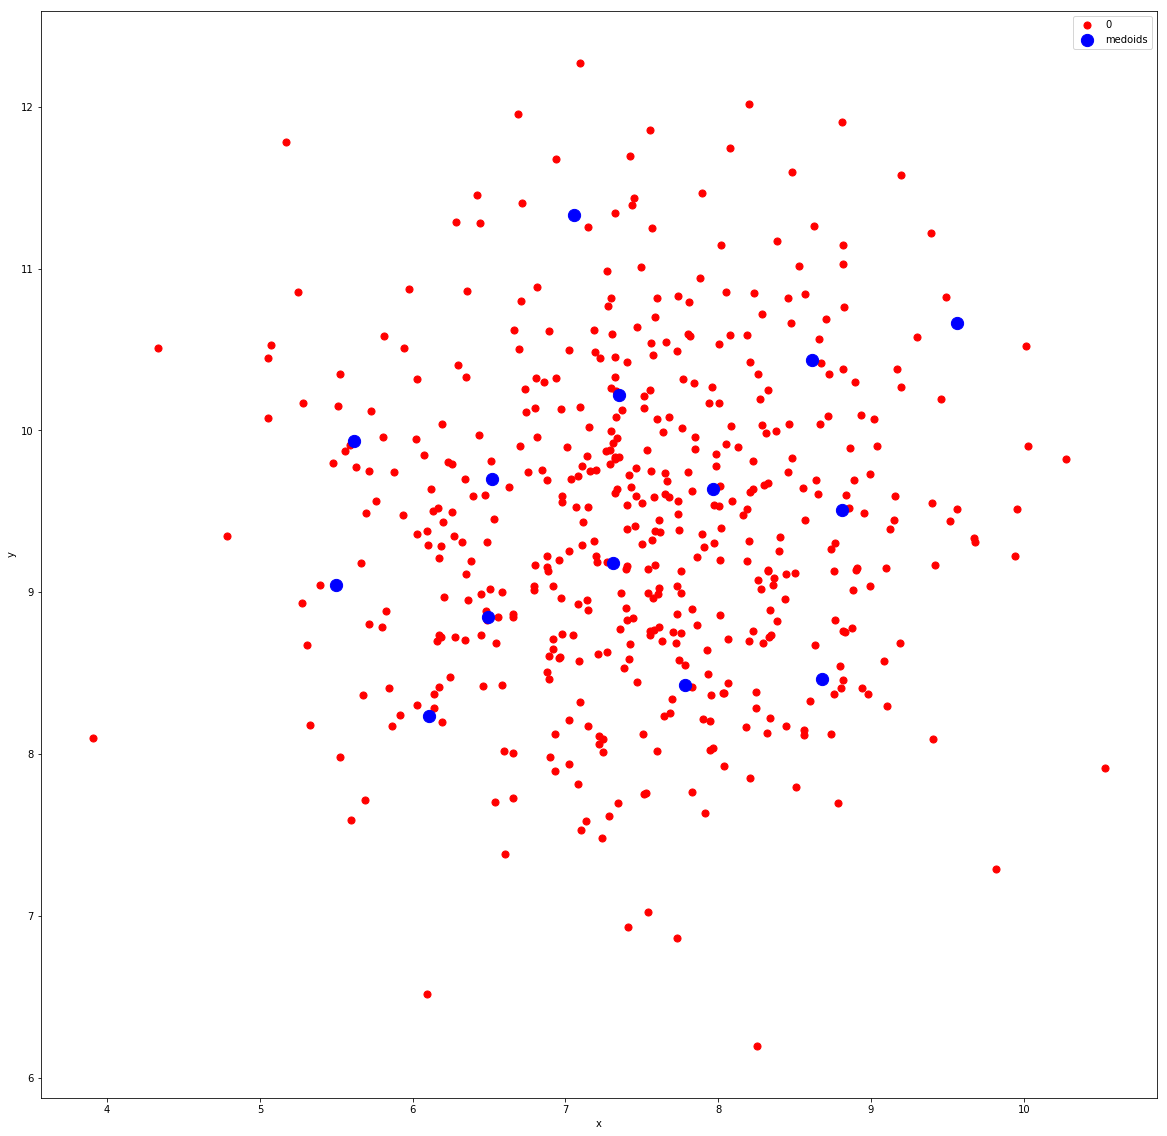
\includegraphics[width=\linewidth]{img/delta_medoids_select_better.png}
  \label{img:blobs_good_select}
  \caption{$\delta$-Medoids choosing only relevant samples of a cluster}
\end{figure}
This sanity check by visualization fulfilled all of the expectation.

\section{Experiment 3}\label{sec:exp3}

After the algorithms were tested on visualizable data, the experiments with well known labeled datasets could start.
The motivation for this experiment was to test the algorithm results on well explored and well-annotated datasets commonly used as a benchmark for clustering.

\subsection{Experimental Setup}
Datasets used for this experiment were:
\begin{itemize}
    \item Pendigit
    \item
\end{itemize}

All 4 algorithms were run.
The $\delta$ was estimated as \todo{how is median at lower ten percent called, put it to maths} times 1.05 from distances from one point in the data to all of the others.

\subsection{Results}

The results for different methods are listed below.

\textbf{Pendigits}

\begin{table}[]
\begin{tabular}{l|lllll}
\hline
 \textbf{Cluster} & \specialcell{\textbf{All}\\ \textbf{Samples}} & \specialcell{\textbf{Greedy}\\ \textbf{Selection}} & \specialcell{\textbf{$\delta$-Medoids}\\ \textbf{One-Shot}} & \specialcell{\textbf{$\delta$-Medoids}\\ \textbf{Full}} & \specialcell{\textbf{Random}\\ \textbf{Selection}} \\ \hline
0 & 780 & 33 & 33 & 33 & 33 \\
1 & 779 & 33 & 41 & 41 & 41 \\
2 & 780 & 17 & 15 & 15 & 15 \\
3 & 719 & 12 & 9 & 9 & 9 \\
4 & 780 & 25 & 24 & 24 & 24 \\
5 & 720 & 25 & 27 & 27 & 27 \\
6 & 720 & 16 & 16 & 16 & 16 \\
7 & 778 & 22 & 20 & 20 & 20 \\
8 & 719 & 75 & 77 & 15 & 15 \\
9 & 719 & 50 & 52 & 13 & 13 \\ \hline
\end{tabular}
\caption{Number of selected representatives for Pendigit dataset}
\end{table}

\begin{figure}
   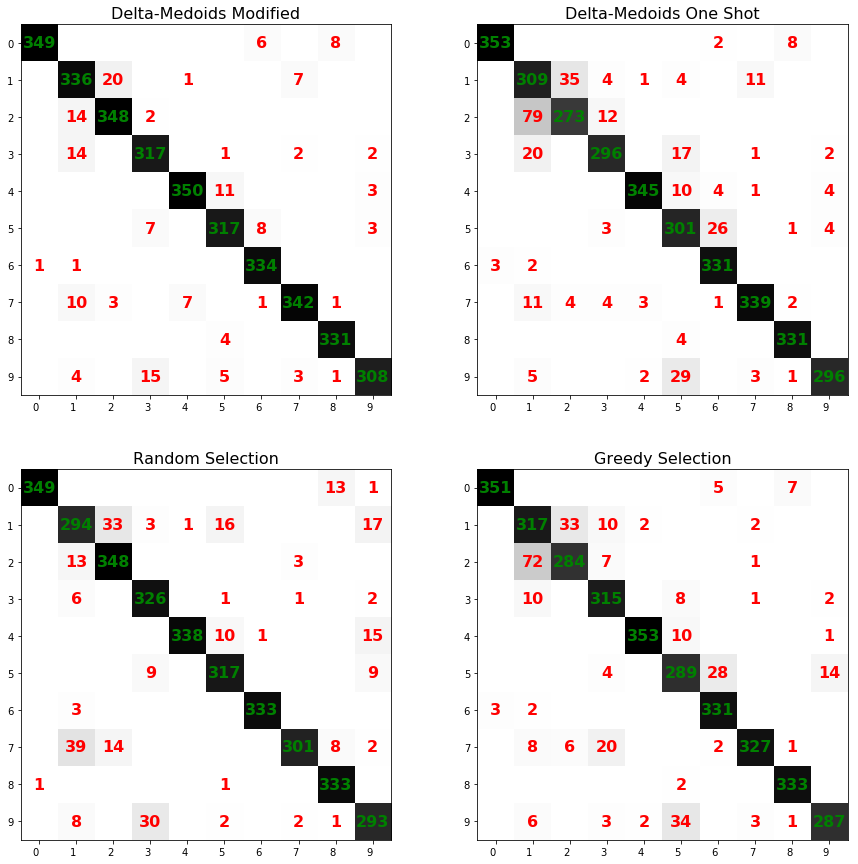
\includegraphics[width=\linewidth]{img/exp3_pendigits.png}
  \label{img:exp3_pendigits}
  \caption{Confusion matrices for Pendigits dataset}
\end{figure}

\subsection{Conclusion}
Using algorithms on real datasets started to show more significant differences between results in algorithms.
An interesting thing is that Greedy Selection and $\delta$-Medoids One-Shot select similar number of representatives and their results are also very similar.
This is interesting as the complexity of these algorithms differs a lot, Greedy Selection being much slower with $\mathcal(n^2)$. \todo{better wording of this conclusion}


\setsecnumdepth{part}

%========================================CHAPTER==================================

\chapter{Conclusion}
Literature in both Network Anomaly Detection field and representative selection was studied.
Approaches and algorithms thus found were combined and implemented in prototype program.
Both general clustering datasets and specific datasets from security field were tested and compared in the prototype. \\

For testing the selected method datasets were created and gathered from the internet to create a diverse testbed for comparing algorithms.
From the selected algorithms both $\delta$-Medoids One Shot and $\delta$-Medoids outperformed Random selection of representatives, which is the current solution of representatives selection in the framework.
The improvement was at least by 1\% in each dataset, while average improvement was 2\%. \todo{Double check these numbers.} \\

\todo{Fine-tune the algorithms for the NBAD field and write here about it if it works.}

If compared by the requirements from the definition of representative selection problem as we approach it, the following can be concluded.
For fast representative selection that does result in more accurate result than selecting samples randomly, $\delta$-Medoids One Shot algorithm should be used.
If the speed is not of great concern or the datastets have lower tens of thousands of samples, full version of $\delta$ medoids yields the best results.

\bibliographystyle{iso690}
\bibliography{hlavac-thesis.bib}

\setsecnumdepth{all}
\appendix

\chapter{Abreviations}
% \printglossaries
\begin{description}
	\item[NIDS] Intrusion Detection System
	\item[NBAD] Network-Based Anomaly Detection
\end{description}


\chapter{Contents of enclosed CD}

%change appropriately

\begin{figure}
	\dirtree{%
		.1 readme.txt\DTcomment{the file with CD contents description}.
		.1 exe\DTcomment{the directory with executables}.
		.1 src\DTcomment{the directory of source codes}.
		.2 wbdcm\DTcomment{implementation sources}.
		.2 thesis\DTcomment{the directory of \LaTeX{} source codes of the thesis}.
		.1 text\DTcomment{the thesis text directory}.
		.2 thesis.pdf\DTcomment{the thesis text in PDF format}.
		.2 thesis.ps\DTcomment{the thesis text in PS format}.
	}
\end{figure}

\end{document}
